%
% Szakdolgozatminta az Eszterházy Károly Katolikus Egyetem
% matematika illetve informatika szakos hallgatóinak.
%

\documentclass[
% opciók nélkül: egyoldalas nyomtatás, elektronikus verzió
% twoside,     % kétoldalas nyomtatás
% tocnopagenum,% oldalszámozás a tartalomjegyzék után kezdődik
]{thesis-ekf}
\usepackage[T1]{fontenc}
\PassOptionsToPackage{defaults=hu-min}{magyar.ldf}
\usepackage[magyar]{babel}
\usepackage{mathtools,amssymb,amsthm,pdfpages}
\footnotestyle{rule=fourth}

\usepackage{listings}
\renewcommand{\lstlistingname}{}

\newtheorem{tetel}{Tétel}[chapter]
\theoremstyle{definition}
\newtheorem{definicio}[tetel]{Definíció}
\theoremstyle{remark}
\newtheorem{megjegyzes}[tetel]{Megjegyzés}

\lstdefinelanguage{TypeScript}{
	language=Java,
	morekeywords={await, async, let, const, type, interface},
	sensitive=true
}

\lstset{
	language=TypeScript,
	basicstyle=\ttfamily\small,
	keywordstyle=\color{blue}\bfseries,
	commentstyle=\color{green},
	stringstyle=\color{red},
	numbers=left,
	numberstyle=\tiny\color{black},
	stepnumber=1,
	breaklines=true,
	frame=single,
	backgroundcolor=\color{lightgray},
	xleftmargin=2.5cm,
	xrightmargin=2.5cm,
	framexleftmargin=5mm,
	framexrightmargin=5mm 
}

\begin{document}

\institute{Matematikai és Informatikai Intézet}
\title{Mesterséges intelligencia számítógépes játékokban}
\author{Budai Roland\\Programtervező informatikus BSc.}
\supervisor{Dr. Kovásznai Gergely\\Egyetemi docens}
\city{Eger}
\date{2024}
\maketitle

\tableofcontents

\chapter*{Bevezetés}
\addcontentsline{toc}{chapter}{Bevezetés}

A szakdolgozatom témája egy stratégiai társasjáték implementálása beépített Mesterséges intelligenciával, amely segít a támadási döntések meghozatalában. A projekt ötlete nem csupán egy tanulmányi kötelezettség teljesítéséből fakad, hanem egy régebb óta tervezett hobbi projekt része is. Már a tanulmányaim elején megfogalmazódott bennem a kérdés, hogy hogyan tudnék egy hasonló társasjátékot a számítógépes világban megvalósítani. Milyen adatbázist kell elkészíteni, milyen döntéseket hozhatnak a játékosok, hogyan lehet megoldani, hogy egyszerre többen is hozzáférjenek az adatokhoz, mégis konzisztens maradjon a játékmenet és a tárolt állapotai a játéknak? Hasonló kérdések fogalmazódtak meg bennem tanulmányaim során, melyekre a képzés ideje alatt egyre jobb és jobb ötleteket sikerült szereznem. Mindezek miatt nagy lelkesedéssel álltam neki a feladatnak a témaválasztást követően. 

További érdekessége a szakdolgozatnak a mesterséges intelligencia (MI) fejlesztése, használata. A mesterséges intelligencia és a gépi tanulás területei egyre nagyobb szerepet játszanak a modern játékfejlesztésben, ezért ez a projekt nemcsak szakmai kihívást jelentett számomra, hanem egyben kiváló lehetőséget is arra, hogy mélyebben megismerkedjek az MI alkalmazásával, fejlesztésével a játékok világában. Az MI implementálásával lehetőségem nyílt egy olyan ellenfél létrehozására, amely képes tanulni és folyamatosan fejlődni a játékok során. 

A mesterséges intelligencia fejlődése az elmúlt években jelentősen befolyásolta a játékfejlesztés folyamatát, lehetővé téve, hogy az MI-alapú ellenfelek egyre intelligensebb döntéseket hozzanak és alkalmazkodjanak a játékosok stratégiájához. Stratégiai döntések meghozatalához különösen a projektemben is használt megerősítéses tanulás (reinforcement learning, RL) vált népszerűvé, amely az MI folyamatos fejlődését, tanulását teszi lehetővé.

\chapter{MI és technológia}

\section{Megerősítéses tanulás elméleti alapjai}

%TODO: gépi tanulás, neurális hálózat, ügynök, környzet fogalmak

A megerősítéses tanulás (Reinforcement Learning, RL) olyan gépi tanulási módszer, amelyben az ügynök egy környezetben interakciók során tanul optimális stratégiákat kialakítani. Az RL egyik legfőbb célja a döntéshozatal optimalizálása egy adott probléma keretein belül. \cite{RL} A megerősítéses tanulás egyik alapvető fogalma az állapot (state, $S$), amely a környezet aktuális reprezentációja, amely leírja az ügynök és a környezet közötti pillanatnyi helyzetet. A cselekvés (action, $A$) az ügynök által végrehajtható lépések halmaza. A jutalom (reward, $R$) a környezet visszacsatolása egy adott cselekvés végrehajtása után. Az ügynök célja ezen jutalom hosszú távon való maximalizálása. Az ügynök által használt politika (policy, $\pi$) egy szabályrendszer, amely meghatározza, hogy egy adott állapotban milyen cselekvést hajtson végre az ügynök. A hosszú távú jutalom várható értékének számításához egy adott állapot és cselekvés kombinációját használja, ez az úgynevezett Q-érték (Q-value, $Q(s,a)$).

Az RL során az ügynök kísérlet és hiba (trial and error) folyamat révén tanulja meg a várhatóan legjobb kimenetelű döntéseket. Számtalan algoritmust használhatunk a tanításhoz, ezek közül a legismertebbek közé tartozik a Q-learning és a Deep Q Nerwork (DQN), amelyek az állapot-cselekvés értékek (Q-értékek) becslésén alapulnak.

Egy stratégiai játékban az RL lehetőséget ad arra, hogy a mesterséges intelligencia adaptálódjon a játékos döntéseihez, és folyamatosan fejlessze saját taktikáját. Az ilyen típusú modellek egyik legfontosabb előnye, hogy nem előre megírt szabályok szerint működnek, hanem a tapasztalatokból tanulnak és fejlődnek.

\section{Felhasznált technológiák}

A projekt megvalósítása során több különböző technológiát alkalmaztam, amelyek lehetővé tették a játék és a mesterséges intelligencia hatékony implementálását. Az MI fejlesztésének alapját a Python nyelv képezte, mivel számos hatékony könyvtár áll rendelkezésre a gépi tanulás számára. A neurális hálózat betanításához és optimalizálásához a PyTorch keretrendszer nyújtott megoldást. A játék backendjének fejlesztéséhez JavaScript-et alkalmaztam, amely lehetővé tette a szerveroldali logikák és az adatkezelés megvalósítását. Az adatokat a dokumentumorientált MongoDB adatbázisban tároltam. A React szolgált egy dinamikus és interaktív frontend fejlesztésére. A szerver és a különböző kliensek közötti kommunikációt kétféleképpen oldottam meg. Az alapvető adatok lekérdezésére REST API-n keresztüli kommunikációt biztosítottam, a valós idejű játékélmény és gyors adatcsere érdekében pedig WebSocket kapcsolatot hoztam létre. További fejlesztési eszközként szolgáltak a GitHub, a Visual Studio Code és az Inkscape amely a frontendhez szükséges svg kiterjesztésű fájlok létrehozásában segített.

\chapter{Játékmechanika}

\section{A játék szabályrendszere és célja}

\section{Játékosok interakciói és fázisai}

\chapter{Implementáció}

\section{Fejlesztési környezet és eszközök}

A projekt fejlesztéséhez Visual Studio Code-ot használok, mivel támogatja mind a Javascript, TypeScript és Python nyelveket, továbbá különböző bővítményekkel egyszerűsíthető a fejlesztési folyamat. Egy ilyen bővítmény például a MongoDB, ami által könnyedén ellenőrizhetjük az adatbázisban történő változások sikerességét. A verziókövetésre a GitHub szolgál, amely lehetővé teszi a változások követését és a biztonságos tárolást, így felváltva tudom fejleszteni a projektet asztali számítógépről és laptopról.

\subsection{Backend}

A játék alapját egy Node.js alapú backend biztosítja, amely a MongoDB adatbázissal kommunikálva tárolja és frissíti a különböző játékállapotokat.

\subsection{Frontend}

A React segítségével épített frontend biztosítja a játékosok számára az interaktív felületet egy webes alkalmazás formájában.

\section{Adatkezelés és játékállapot tárolása}

A játék egyik legfontosabb eleme a játékállapot pontos eltárolása, amely biztosítja a játékosok számára a legfrissebb helyzeteket. Ezáltal az adatbázis tervezése volt az egyik legfontosabb feladat az implementáció során. 

A projektben MongoDB-t használok, mivel ez egy NoSQL-alapú, dokumentum-orientált adatbázis. JSON-szerű dokumentumokat használ, amik könnyedén lekérdezhetők, kezelhetők és bővíthetők, ezáltal jól illeszkednek a játékstruktúrához. \cite{MongoDB} A játékállapot folyamatos frissítése során fontos biztosítani, hogy ne történjenek ütközések, illetve adatvesztések. Ennek biztosítására kínál lehetőséget a MongoDB az Atomic Update műveletekkel, mint például az updateOne() és findOneAndUpdate() beépített függvények.

\lstinputlisting[caption={Példa az Atomic Update műveletekre a cardsService.ts-ből.}, label=kod-atomic-update, captionpos=b]{atomicUpdate.ts}

Hat adatbázis-kollekció lett létrehozva, a következőképpen (lásd: \ref{collections}~ábra):

\begin{figure}[ht!]
	\centering
	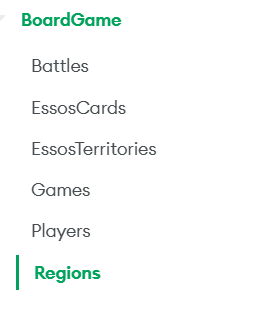
\includegraphics[width=5cm]{Collections.png}
	\caption{A MongoDB-ben tárolt kollekciók.}
	\label{collections}
\end{figure}

\begin{itemize}
	\item \textbf{Players}: a játékosok adatait tartalmazza
	\item \textbf{Games}: az aktuális és lezárt játszmák állapotát tartalmazza
	\item \textbf{Territories}: a térkép területeit és kapcsolataikat írja le
	\item \textbf{Cards}: a játékban szereplő kártyák helyzetét rögzíti
	\item \textbf{Regions}: a területeket összekötő régiókat tartalmazza
	\item \textbf{Battles}: a folyamatban lévő és lezárt csaták részleteit kezeli
\end{itemize}

A játék adatbázisának célja, hogy hatékonyan kezelje a játékállapotot, a területek, a játékosokat, a kártyákat és a csatákat. Az alábbiakban részletesen bemutatom az egyes táblák szerepét, a közöttük lévő kapcsolatokat, valamint az adatok kezelésének menetét. A régiókat tartalmazó kollekció a Regions.csv-ből került betöltésre, azonban mivel ezek az adatok nem változnak játék közben és két játék között sem, ezért ezzel a táblával adatmódosítás szempontjából nem is kell foglalkozni. Fő célja a kör elején kapott bónusz seregek számításánál a régióbónusz meghatározása. Erre a calculatePlusArmies(playerId: ObjectId) metódusban kerül sor (\ref{region-bonus}).

\lstinputlisting[caption={Régióbónusz meghatározása.}, label=region-bonus, captionpos=b]{regionBonus.ts}

Egy új játék elkezdésénél elsősorban a Games kollekció került módosításra. A state mezője felel a játék státuszának követésében, háromféle értéket vehet fel: ongoing, azaz ez a játék még éppen folyamatban van, terminated, miszerint a játék valamilyen oknál fogva befejeződött, le lett zárva a szerver által és X won, ahol az X a győztes játékos házának neve. Amikor valaki elindít egy új játékot, akkor a szerver megnézi, hogy van-e folyamatban lévő játék, és ha van, akkor azt lezárja, majd létrehoz egy új példányt egyedi azonosítóval és a kört 1-re állítja.

Ezután következik a kártyák betöltése a seedEssosCards() függvénnyel és ezek megkeverése a shuffle() függvénnyel. Hasonlóan a régiókhoz, a kártyák is egy csv-ből kerülnek az adatbázisba, azonban a kártyák minden játék elején újratöltődnek. Minden kártyánál beállításra kerül a játékazonosító mező az előtte létrehozott új játék azonosítójával, illetve a tulajdonos mező "in deck" azaz a pakliban értéket vesz fel. A shuffle() biztosítja, hogy a kártyák véletlenszerűen legyenek elhelyezve a pakliban (a játék vége kártya is itt van biztosítva, hogy ne kerülhessen elő túl hamar, lásd \ref{game-end-card}~ábra).

\lstinputlisting[caption={A játék vége kártya helyének biztosítása.}, label=game-end-card, captionpos=b]{GameEndCard.ts}

Miután minden kártya a helyére került, a generatePlayers(numberOfPlayers: number) függvény kerül meghívásra. A függvény létrehozza a kívánt mennyiségű játékost és betölti őket az adatbázisba, majd a Games kollekcióban módosításra kerül a players tömb, belekerülnek az újonnan létrehozott játékosok házainak nevei.

Végezetül a területek kerülnek az adatbázisba a seedEssosTerritories() függvénnyel. A függvény csak betölti a területekhez tartozó általános adatokat, az allocateTerritories() függvény felel a terület birtokosának meghatározásában. Ez a függvény két játékos között osztja szét a területeket a következőképpen: 12 véletlenszerűen választott területet kap az első játékos, 12 területet a második és a maradék terület birtokosa a semleges értéket kapja. Mindezek után az első játékos megkapja a neki járó plusz seregeket és kezdődhet is a játék.

Egyetlen kollekció van, amely egy új játék létrehozásánál nem játszik semmilyen szerepet, a csatákat tartalmazó tábla. Ez a kollekció felel a már lejátszott és a még zajló csaták nyomon követésében. Amikor egy csata létrejön, akkor beállításra kerülnek az alapvető mezők mint például a támadó azonosítója, vagy a védekező terület azonosítója a szerver által. A csata közben a kör száma mező módosul, a dobások értékeinek mezője, illetve a csatanapló. Ha egy csatának vége van, akkor az állapota módosul az egyik fél győzelmére, majd a csatanaplóban lehet visszanézni, hogy pontosan hogyan is ment végbe az adott csata.

%TODO: adatbázis képet beletenni

\chapter{Mesterséges intelligencia tervezése}

\section{Kommunikáció a szerverrel}

\section{Környezet tervezése}

\section{Tanítás és fejlesztés}

\chapter{Az elkészült alkalmazás}

\section{Tanítás eredménye, pontosság, hiba mértéke}

\section{TEMP: elkészült alkalmazásról képek?}

\chapter*{Összegzés}
\addcontentsline{toc}{chapter}{Összegzés}

\begin{thebibliography}{2}
\addcontentsline{toc}{chapter}{\bibname}
\bibitem{Tomacs}
\textsc{Tómács Tibor}: \emph{A valószínűségszámítás alapjai}, Líceum Kiadó, Eger, 2005.
\bibitem{RL}
\textsc{Reinforcement Learning wikipedia}: https://en.wikipedia.org/wiki/Reinforcement\_learning
\bibitem{MongoDB}
\textsc{MongoDB wikipedia}: https://en.wikipedia.org/wiki/MongoDB
\end{thebibliography}

% Aláírt, szkennelt nyilatkozat beillesztése a szakdolgozat végére
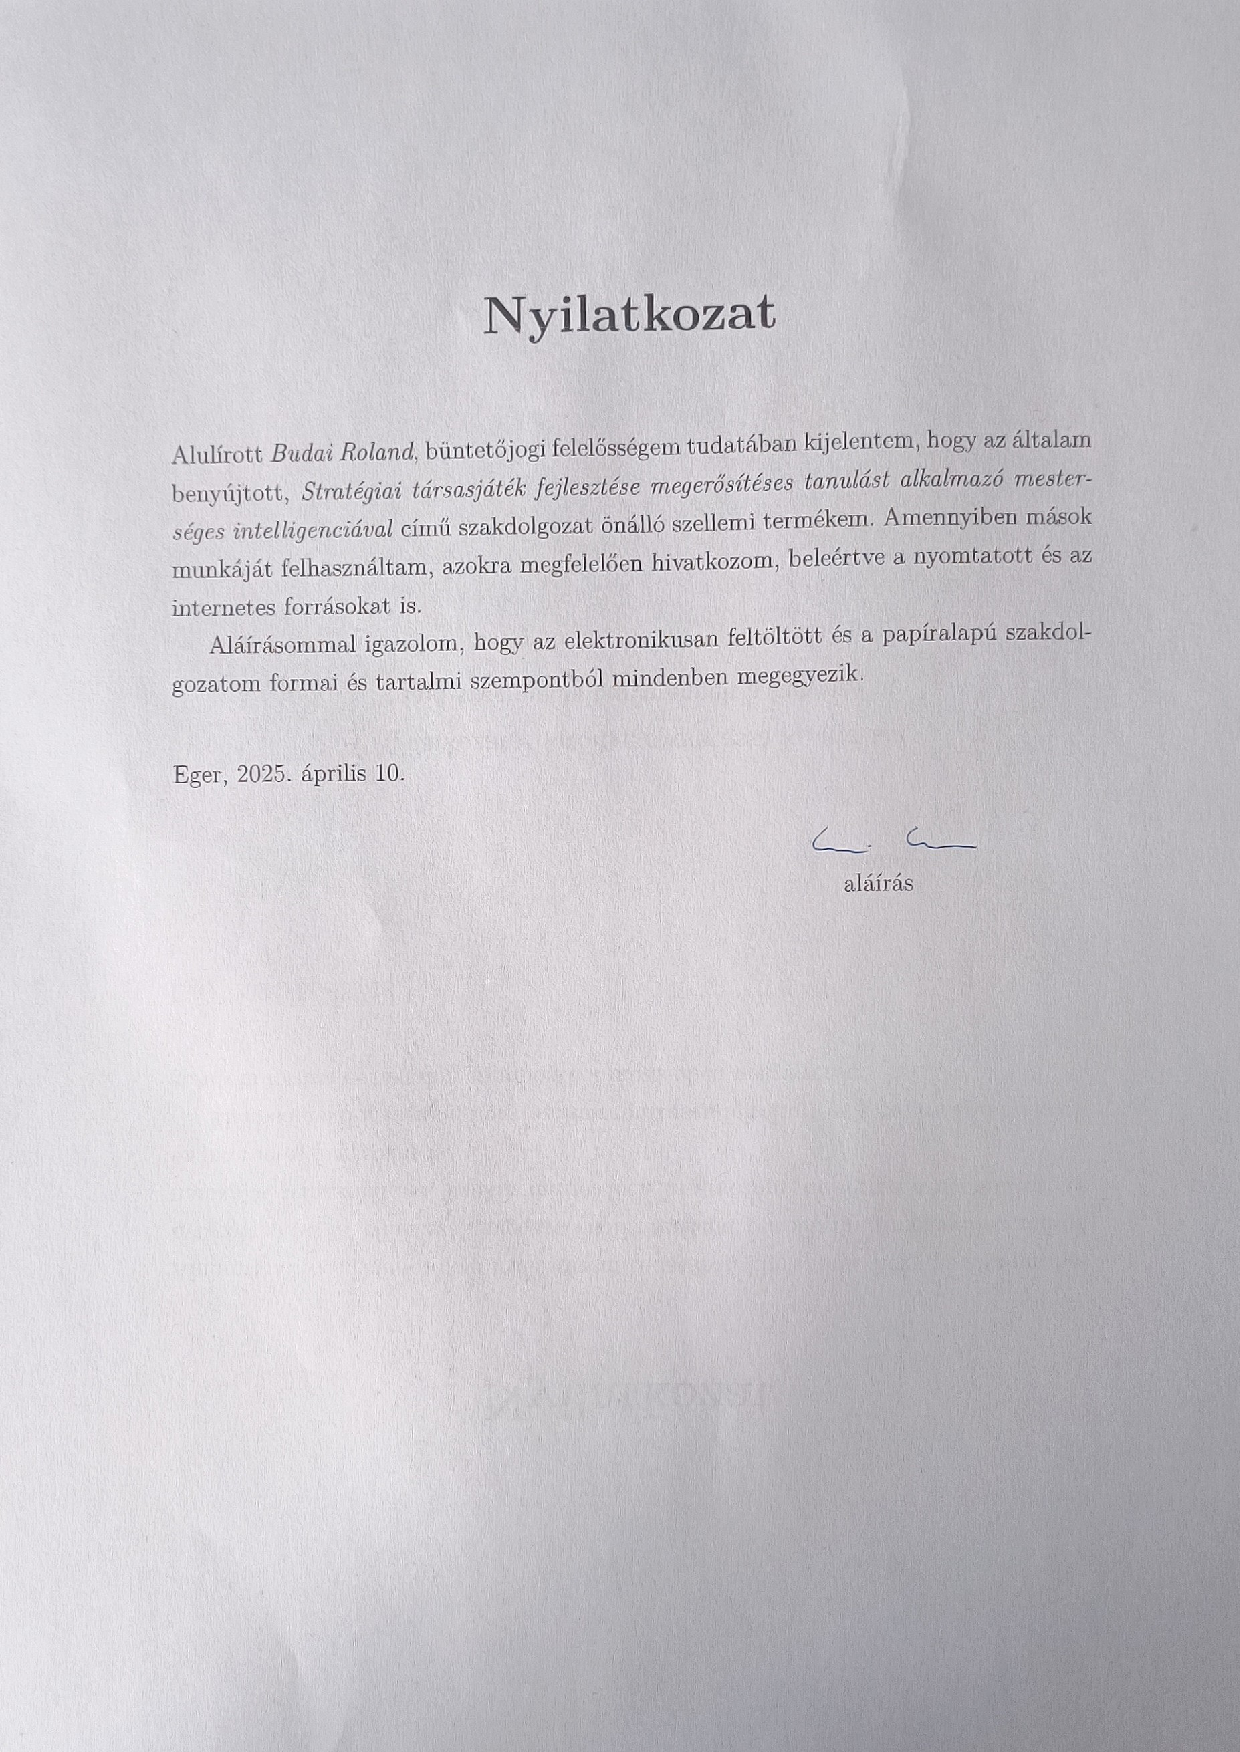
\includepdf{nyilatkozat.pdf}

\end{document}